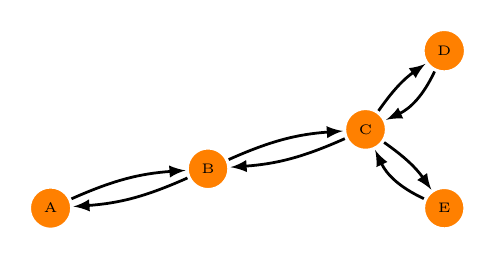
\begin{tikzpicture}[font=\tiny]
    \tikzstyle{node_style} = [draw=white, very thick, circle, fill=orange]
    \tikzstyle{arrow_style1} = [->, black, line width=1, >=latex]

    \node[node_style] (n1) at (0,0) {A};
    \node[node_style] (n2) at (2,0.5) {B};
    \node[node_style] (n3) at (4,1) {C};
    \node[node_style] (n4) at (5,2) {D};
    \node[node_style] (n5) at (5,0) {E};

    \draw[arrow_style1] (n1) edge [bend left=10] (n2);
    \draw[arrow_style1] (n2) edge [bend left=10] (n1);
    \draw[arrow_style1] (n2) edge [bend left=10] (n3);
    \draw[arrow_style1] (n3) edge [bend left=10] (n2);
    \draw[arrow_style1] (n3) edge [bend left=10] (n4);
    \draw[arrow_style1] (n4) edge [bend left=20] (n3);
    \draw[arrow_style1] (n3) edge [bend left=10] (n5);
    \draw[arrow_style1] (n5) edge [bend left=20] (n3);
    %\draw[arrow_style3, shorten <=2pt, shorten >=2pt] (n2) edge [out=140, in=-60] (n4);
\end{tikzpicture}
